%!TEX root = ../template.tex
%%%%%%%%%%%%%%%%%%%%%%%%%%%%%%%%%%%%%%%%%%%%%%%%%%%%%%%%%%%%%%%%%%%%
%% chapter4.tex
%% NOVA thesis document file
%%
%% Chapter with lots of dummy text
%%%%%%%%%%%%%%%%%%%%%%%%%%%%%%%%%%%%%%%%%%%%%%%%%%%%%%%%%%%%%%%%%%%%

\typeout{NT FILE chapter4.tex}%

\chapter{Tool Design for Blade Clearance Control}
\label{cha:toolclear}


Following the conclusions drawn in Section~\ref{cha:contacto} regarding the actual contact points between blade platforms, this chapter focuses on applying reverse engineering to determine the chord length of the blade platforms and . The approach involves analyzing the contact zones identified previously and determine the correct platform chord dimensions. Furthermore, the diameters of the spool will be determined by opening a case with the manufacturer to request these specific dimensions, ensuring accuracy in the assembly process.

With this information, the chapter proceeds to the design of a tool for blade clearance control, capable of assessing the contact clearance between the blades during assembly. The tool will be designed based on nominal tolerances, estimated blade configurations, and the dimensional analysis of the spool diameter, ensuring precise control over the final assembly clearance.


\section{Statistical Analysis for Tolerance Estimation}

The first step in this process is determining how many blades need to be measured in order to obtain a credible and accurate chord dimension. 
To assess this, a statistical methodology was applied. Since no manufacturing tolerances were provided, these were estimated based on direct measurements performed with a caliper. 
The approach is grounded in standard principles of statistical quality control and process capability analysis, as detailed in Requeijo and Pereira's work on process planning and statistical control.

\subsection{Sampling Strategy}

Building upon the methodology, the next step is to determine the number of blades to be measured from each stage to ensure reliable results. 
A pilot sample was used to estimate the required number of measurements for process characterization.
Six used blades were measured per stage using a digital caliper. The results for stages 6 to 10 are presented in Table~\ref{tab:pilot_measurements}.
As shown in Figure~\ref{fig:corda}, the dimension "x" represents the chord length being measured on the blade platform.

\begin{figure}[H]
    \centering
    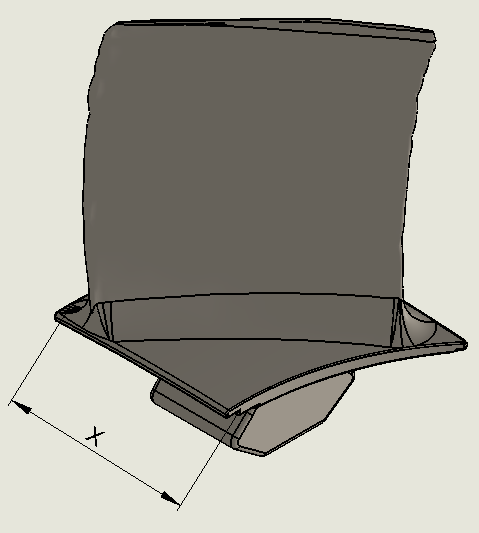
\includegraphics[width=0.4\textwidth]{corda}
    \caption{Platform blade with the chord dimension being measured, indicated as "x".}
    \label{fig:corda}
\end{figure}

\begin{table}[H]
    \centering
    \caption{Pilot measurements of platform chord lengths (mm) for stages 6 to 10.}
    \label{tab:pilot_measurements}
    \begin{tabular}{ccccc}
        \hline
        \textbf{Stg 6} & \textbf{Stg 7} & \textbf{Stg 8} & \textbf{Stg 9} & \textbf{Stg 10} \\
        \hline
        18.71 & 20.37 & 18.59 & 19.48 & 18.26 \\
        18.71 & 20.36 & 18.58 & 19.49 & 18.28 \\
        18.72 & 20.37 & 18.61 & 19.46 & 18.28 \\
        18.72 & 20.36 & 18.58 & 19.47 & 18.26 \\
        18.71 & 20.36 & 18.59 & 19.48 & 18.28 \\
        18.72 & 20.37 & 18.57 & 19.48 & 18.28 \\
        \hline
    \end{tabular}
\end{table}

Using this data, the required sample size \(n\) for a given confidence level of and measurement precision was determined using the expression:

\[
n = \left( \frac{Z \cdot s}{E} \right)^2
\]

Where:
\begin{itemize}
    \item \(Z\): standard normal value for the chosen confidence level (in this case 1.96 for 95\% of confidence),
    \item \(s\): standard deviation estimated from the pilot sample,
    \item \(E\): maximum acceptable error (typically set to 0.01 mm, matching the caliper's resolution).
\end{itemize}

The values of \(s\) and the corresponding sample sizes for each stage are presented in Table~\ref{tab:sample_sizes_data} for the narrow body type blades and on Table~\ref{tab:sample_sizes_data_wide} for the wide body type blades.

\begin{table}[H]
    \centering
    \caption{Calculated sample sizes for Narrow Body blades based on standard deviation from pilot sample, confidence level, and maximum error.}
    \label{tab:sample_sizes_data}
    \begin{tabular}{cccc}
        \hline
        \textbf{s} & \textbf{Z} & \textbf{E} & \textbf{n} \\
        \hline
        0.006956076 & 1.96 & 0.005 & 7 \\
        0.006956076 & 1.96 & 0.005 & 7 \\
        0.013319872 & 1.96 & 0.005 & 27 \\
        0.013116504 & 1.96 & 0.005 & 26 \\
        0.006558252 & 1.96 & 0.005 & 7 \\
        \hline
    \end{tabular}
\end{table}

\begin{table}[H]
    \centering
    \caption{Calculated sample sizes for Wide Body blades based on standard deviation from pilot sample, confidence level, and maximum error.}
    \label{tab:sample_sizes_data_wide}
    \begin{tabular}{cccc}
        \hline
        \textbf{s} & \textbf{Z} & \textbf{E} & \textbf{n} \\
        \hline
        0.006956076 & 1.96 & 0.005 & 7 \\
        0.006956076 & 1.96 & 0.005 & 7 \\
        0,016558774 & 1.96 & 0.005 & 42 \\
        0,010625582 & 1.96 & 0.005 & 17 \\
        0,005679613 & 1.96 & 0.005 & 5 \\
        \hline
    \end{tabular}
\end{table}


Regarding the number of measurements per blade, only one measurement was taken per blade. 
This choice is justified by the high resolution of the caliper, which is calibrated, and the repeatability of the measurement procedure, with measurements consistently performed by a single operator. 
According to principles described in the literature, and particularly by Requeijo and Pereira, when the measurement system is precise and the method is consistent, a single measurement per part is acceptable in statistical process control. 
Repeated measurements are mostly recommended when evaluating the measurement system itself (e.g., during a repeatability and reproducibility study).

\subsection{Estimating Process Tolerance}

Knowing the number of measurements needed per stage, the following step is measuring new \gls{HPC} blades available on \gls{TAP}'s engine shop.
For each blade group, the sample mean \(\bar{x}\) and standard deviation \(s\) were computed. Assuming normality in the data distribution, the process tolerance can estimated as:

\[
T = 6s
\]

According to literature this range is expected to encompass approximately 99.73\% of blades, reflecting a standard tolerance interval associated with normally distributed processes.

Example for wide blades from stage 7:

\begin{itemize}
    \item Measurements: \{20.62, 20.62, 20.61, 20.62, 20.62, 20.62, 20.61\} mm
    \item Mean: \(\bar{x} = 20.6171\) mm
    \item Standard deviation: \(s = 0.00488\) mm
    \item Tolerance estimate: \(T = 0.02928\) mm
\end{itemize}

Tables~\ref{tab:mean_tolerance_narrow} and~\ref{tab:mean_tolerance_wide} present all the measurement results and estimated tolerances for each stage.

\begin{table}[H]
    \centering
    \caption{Sample mean and tolerance estimates for each stage of the Narrow Body blades.}
    \label{tab:mean_tolerance_narrow}
    \begin{tabular}{cccc}
        \hline
        \textbf{Stage} & \multicolumn{3}{c|}{\textbf{Narrow Body}} \\
        \hline
        & \textbf{Mean (\( \bar{x} \))} & \textbf{Standard Deviation (\( s \))} & \textbf{Tolerance Estimate (\( T = 6s \))} \\
        \hline
        6  &  &  &  \\
        7  & 20.374 & 0.005345 & 0.032 \\
        8  & 18.591 & 0.007863  & 0.047 \\
        9  & 19.490 & 0.006939  & 0.042 \\
        10 & 18.284 & 0.005345  & 0.032 \\
        \hline
    \end{tabular}
\end{table}

\begin{table}[H]
    \centering
    \caption{Sample mean and tolerance estimates for each stage of the Wide body blades.}
    \label{tab:mean_tolerance_wide}
    \begin{tabular}{cccc}
        \hline
        \textbf{Stage} & \multicolumn{3}{c|}{\textbf{Wide Body}} \\
        \hline
        & \textbf{Mean (\( \bar{x} \))} & \textbf{Standard Deviation (\( s \))} & \textbf{Tolerance Estimate (\( T = 6s \))} \\
        \hline
        6  & 18.984 & 0.00535 & 0.032 \\
        7  & 20.617 & 0.00488 & 0.029 \\
        8  & 18.846 & 0.0059  & 0.035 \\
        9  & 19.753 & 0.00488  & 0.029 \\
        10 & 18.534 & 0.00548  & 0.033 \\
        \hline
    \end{tabular}
\end{table}


As discussed in Section~\ref{subsec:desafios}, the tolerance allowed for each blade at each stage, as shown in Table~\ref{tab:clearance}, is always larger than the tolerance estimated in this chapter, making it a solid and admissible estimation. Thus, it can also be concluded that the nominal chord length of the blade platform corresponds to the mean value presented in the tables.

Considering the mass production of these blades, and as previously mentioned, these tolerances must be analyzed through the statistical method. This approach assumes that the measurements of a specific dimension within a batch of parts follow a normal distribution. By analyzing, for example, an engine assembled in the workshop, and considering the number of wide, narrow, and lock blades per stage, it is possible to assess the potential dimensional variation of the blade set. The number of blades assembled per stage, as shown in Table~\ref{tab:number_of_blades}, provides a clear overview of the blade distribution, which is essential for understanding the dimensional variability in the assembly process.

\begin{table}[H]
    \centering
    \caption{Number of Wide, Narrow, and Lock Blades per Stage}
    \label{tab:number_of_blades}
    \begin{tabular}{cccc}
        \hline
        \textbf{Stage} & \textbf{Wide Blades} & \textbf{Narrow Blades} & \textbf{Lock Blades} \\
        \hline
        Stg 6 & 36 & 22 & 4 \\
        Stg 7 & 33 & 20 & 4 \\
        Stg 8 & 39 & 20 & 4 \\
        Stg 9 & 37 & 19 & 4 \\
        Stg 10 & 38 & 22 & 4 \\
        \hline
    \end{tabular}
\end{table}

\begin{equation}
\text{TolC} = \sqrt{T_N^2 \cdot (N + L) + T_W^2 \cdot W}
\end{equation}

Where:
\begin{itemize}
    \label{eq:tolc}
    \item \( T_N \) is the tolerance associated with both narrow and lock blades (same value).
    \item \( N \) is the number of narrow blades.
    \item \( L \) is the number of lock blades.
    \item \( T_W \) is the tolerance associated with wide blades.
    \item \( W \) is the number of wide blades.
    \item \( \text{TolC} \) represents the total combined tolerance, taking into account the individual tolerances of both narrow and wide blades, as well as the number of blades of each type.
\end{itemize}

Applying equation~\ref{eq:tolc}, it is possible to evaluate whether the total dimensional variation at each stage remains within acceptable limits for the assembly process. 
Table~\ref{tab:dimensional variation} presents the calculated dimensional variation for each stage, showing a significant deviation in Stage 6, followed by substantially lower and consistent values in the subsequent stages, suggesting a stable manufacturing process.


\begin{table}[H]
    \centering
    \caption{Total dimensional variation per stage}
    \label{tab:dimensional variation}
    \begin{tabular}{cc}
        \hline
        \textbf{Stage} & \textbf{Dimensional Variation} \\
        \hline
        Stg 6 &         \\
        Stg 7 &  0.239  \\
        Stg 8 & 0.263   \\
        Stg 9 & 0.237   \\
        Stg 10 & 0.268  \\
        \hline
    \end{tabular}
\end{table}

\subsection{Conversion from Chord to Arc}

Before defining the dimensions of the blade clearance control tool, it is essential to convert the measured platform chord length into the corresponding arc length, as the actual contact between the blades occurs along the circumference of the engine's spool perimeter.

Assuming a circular geometry, the relation between the chord \(c\), arc length \(a\), and radius \(R\) is given by:

\[
a = R \cdot \theta = 2R \cdot \arcsin\left( \frac{c}{2R} \right)
\]

Where:
\begin{itemize}
    \item \(c\): chord length of the platform,
    \item \(R\): radius of the stage perimeter,
    \item \(a\): arc length corresponding to that chord.
\end{itemize}

In practice, for small angles and short chords the chord and arc are approximately equal. 
However, to ensure dimensional precision in the tool design, the arc length is computed using the actual measured chord and known stage radius.

\begin{table}[H]
    \centering
    \caption{Chord and Tolerance for Each Stage (Wide and Narrow)}
    \label{tab:chord_tolerance_per_stage}
    \begin{tabular}{ccccc}
        \hline
        \textbf{Stage} & \multicolumn{2}{c}{\textbf{Wide}} & \multicolumn{2}{c}{\textbf{Narrow}} \\
        \hline
         & \textbf{Arc length (mm)} & \textbf{Tolerance (mm)} & \textbf{Arc lenght (mm)} & \textbf{Tolerance (mm)} \\
        \hline
        6 & 20.383 & 0.032 & 18.992 & 0.032 \\
        7 & 20.383 & 0.032 & 20.626 & 0.029 \\
        8 & 18.598 & 0.030 & 18.853 & 0.031 \\
        9 & 19.498 & 0.030 & 19.761 & 0.029 \\
        10 & 18.291 & 0.032 & 18.541 & 0.033 \\
        \hline
    \end{tabular}
\end{table}


\subsection{Spool diameter Tolerancing}

In order to accurately define the measurement process of the blade platforms, it is also essential to consider the potential dimensional variation of the spool on which the blades are mounted. 
Since this component is not readily available in large quantities at the TAP engine maintenance facility, only two spools were available throughout the course of this dissertation. 
The measurements were taken on the blade platform side of the spool, specifically in the region where blade-to-blade contact occurs, as illustrated in Figure~5.3 and referred to as the Diameter Up.

\begin{table}[H]
    \centering
    \caption{Spool measurements for engines 418 and 463}
    \label{tab:spool_measurements}
    \begin{tabular}{cc|cc}
        \hline
        \multicolumn{2}{c|}{\textbf{in}} & \multicolumn{2}{c}{\textbf{mm}} \\
        \textbf{418} & \textbf{463} & \textbf{418} & \textbf{463} \\
        \hline
        15.550 & 15.550 & 394.970  & 394.970  \\
        15.615 & 15.615 & 396.621  & 396.621  \\
        15.677 & 15.677 & 398.1958 & 398.1958 \\
        15.704 & 15.705 & 398.8816 & 398.9070 \\
        15.690 & 15.688 & 398.5260 & 398.4752 \\
        \hline
    \end{tabular}
\end{table}

Given that only two components were available, it was not possible to carry out a statistical analysis similar to the one performed for the blades. As such, a fundamental tolerance grade was assumed to define the dimensional variation of the spool, based on tolerances applied to diameter-related dimensions in other critical components.

For example, in the case of the \gls{LPT} shaft, although the exact manufacturing dimensions are not available, the operational limits provided by the manufacturer are known. For this part, the inner diameters have an operational tolerance of 0.004 mm, which implies that the manufacturing tolerance must be even tighter to ensure the part remains functional under operating conditions. Assuming a safety factor of 2, a manufacturing tolerance of 0.002 mm can be considered reasonable.

By consulting the table of fundamental tolerances and noting that this diameter falls within the range of 180 mm to 250 mm, it corresponds to an IT01 grade, the tightest standard tolerance for that size range. This demonstrates the high level of manufacturing precision achievable by the supplier.

Taking this into account, it is reasonable to adopt an IT grade for the spool diameter in order to address the dimensional variation in the absence of a sufficiently large sample size. By assuming an IT3 classification, which is considerably less strict than the tolerance estimated for the \gls{LPT} shaft, the spool diameters can be associated with a manufacturing tolerance of approximately 0.013 mm.

The corresponding nominal dimensions and assumed tolerances are presented in Table~\ref{tab:spool_nominal_tolerance}.

\begin{table}[H]
    \centering
    \caption{Nominal spool diameters and assumed manufacturing tolerance (IT3)}
    \label{tab:spool_nominal_tolerance}
    \begin{tabular}{cc}
        \hline
        \textbf{Nominal Diameter [mm]} & \textbf{Tolerance [mm]} \\
        \hline
        394.970 & ±0.0065 \\
        396.621 & ±0.0065 \\
        398.1958 & ±0.0065 \\
        398.8816 & ±0.0065 \\
        398.5260 & ±0.0065 \\
        \hline
    \end{tabular}
\end{table}


\section{Tool Design}

Building on the conclusions drawn from the statistical analysis of the blade platforms in the previous section, this chapter addresses the design of a tool for controlling blade clearance. 
The primary objective of this tool is to measure the sum of the chord lengths of all blades per stage, facilitating the prediction of whether the assembled set meets the required clearance for optimal operation, in accordance with the established operational limits.

The design process will incorporate nominal tolerances, estimated blade configurations, and dimensional analysis of the spool diameter, guaranteeing accurate control over the final clearance during assembly.

\subsection{Material}

The aim of this section is to determine the material to be used for manufacturing the tool, which will be machined on a CNC machine. In order to make an informed decision, several factors must be considered, including cost, weight, and machinability.

The selection of aluminum for the tool is based on its superior machinability, reduced tool wear, and high-speed cutting capability compared to steels and other harder materials. 
Aluminum allows significantly higher cutting speeds while maintaining good dimensional accuracy and excellent surface finish. Its lower hardness, high thermal conductivity, and resistance to built-up edge formation make it ideal for processes where precision and surface integrity are critical. 
Furthermore, its widespread availability and compatibility with various surface treatments make it an economically efficient and technically versatile material for tooling applications \cite{Rahman2023AluminumMachinability}.

Among the available aluminum alloys, the 6000 series is highlighted in the literature as offering a favorable balance between strength, corrosion resistance, and machinability. 
Specifically, alloy 6061 is identified as a reliable option due to its good mechanical properties and consistent cutting behavior, making it a suitable and well-established choice for both structural and precision-machined components \cite{Rahman2023AluminumMachinability}.

Although PTFE (Teflon) was also considered as an alternative material, a comparison of the component weights shows that the aluminum version weighs 7168.82 grams, while the PTFE version weighs 6159.88 grams. 
The relatively small difference in mass demonstrates that the aluminum tool remains light enough to be easily handled and transported by the operator, while offering significantly better mechanical robustness and durability compared to PTFE.


\section{Design Considerations}

One of the key aspects to consider when defining the most suitable tool design is the geometry of the dovetail sections of the blades. 
Since the blades are secured to the tool via these dovetail interfaces, their dimensional characteristics play a critical role in ensuring a proper fit and functional engagement.

To characterize this geometry, ten blades were measured from each stage. For each blade, four key dimensions of the dovetail were recorded: A, B, C, and D. 
These correspond respectively to the upper width, lower width, total height, and lateral offset of the dovetail profile.


\begin{figure}[H]
\centering
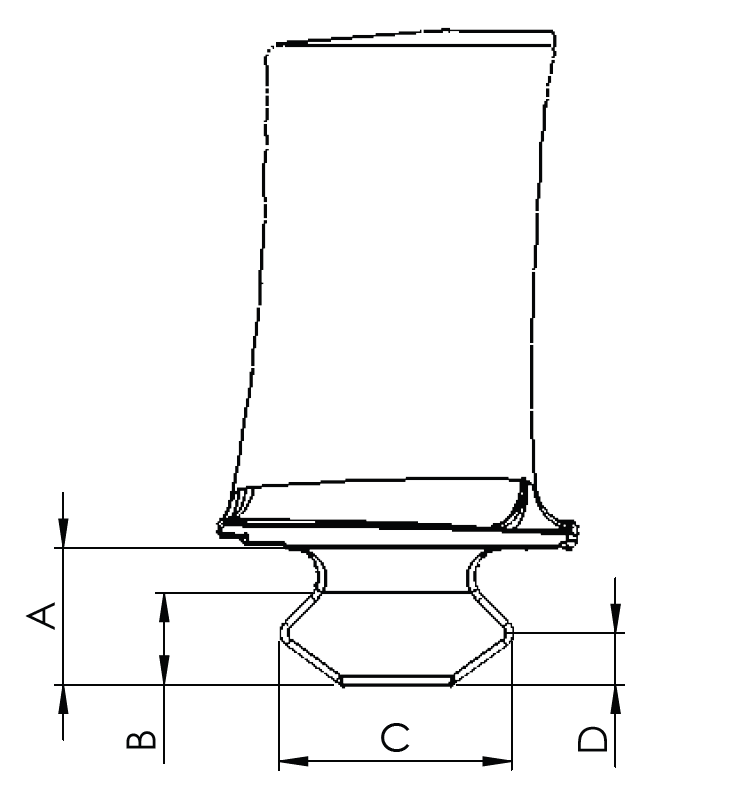
\includegraphics[width=0.6\textwidth]{dovetaildim}
\caption{Schematic representation of the dovetail geometry and its key dimensions (A, B, C, D).}
\label{fig:dovetails}
\end{figure}

Figure~\ref{fig:dovetails} illustrates the progressive variation in dovetail geometry across different stages of the system. 
The dimensions labeled A, B, C, and D refer respectively to the upper width, lower width, height, and lateral offset of each dovetail segment. 


Table~\ref{tab:dovetail_dimensions} summarizes the measured values for each geometric parameter from stage 6 to stage 10. 
As observed, dimension A decreases consistently from 8.20 mm at stage 7 to 6.70 mm at stage 10, indicating a narrowing of the top surface. Similarly, dimension C (height) follows a downward trend, supporting a compact design. 
Dimension B and D exhibit more variability, potentially reflecting design adaptations for mechanical engagement or alignment tolerance.

\begin{table}[H]
    \centering
    \caption{Dovetail dimensions across different stages}
    \label{tab:dovetail_dimensions}
    \begin{tabular}{ccccc}
        \hline
        \textbf{Stage} & \textbf{A (mm)} & \textbf{B (mm)} & \textbf{C (mm)} & \textbf{D (mm)} \\
        \hline
        6  & --   & --   & --    & --    \\
        7  & 8.20 & 4.90 & 13.60 & 2.70  \\
        8  & 7.70 & 5.30 & 12.70 & 1.80  \\
        9  & 6.90 & 4.15 & 11.00 & 1.90  \\
        10 & 6.70 & 4.73 & 10.20 & 2.10  \\
        \hline
    \end{tabular}
\end{table}

The engagement between the blade and the tool is defined by dimension C. Therefore, the fit between both parts must be carefully selected to ensure accurate chord measurements. 
The goal is to allow the blades to be inserted manually into the tool and to slide along it with minimal resistance, while still limiting excessive clearance that could compromise the accuracy of the measurements. 
According to \cite{TabelaAjustesMecanicos}, for medium mechanical precision and a sliding fit, the recommended tolerances are H8 for the hole and h8 or h9 for the shaft.

In addition to the dovetail geometry, another critical consideration in the design of the tool is the definition of the operational limits for the sum of the blade chords within the slot. These limits are essential for establishing the acceptable dimensional range to be used during blade inspection and tool setup.

To define these operational limits, a combined reasoning approach was followed:

Firstly, the dimensional variation of the spool was considered. 
By analyzing the maximum and minimum values of the spool perimeter (Pmax and Pmin) for each stage, and subtracting the maximum and minimum admissible clearances, a functional tolerance window was obtained. 
This defines the upper and lower bounds for the sum of blade chords to be accepted within the tool.

Secondly, it was necessary to account for the geometric transition from arc to chord. 
In the engine, blades are arranged along a circular arc, whereas in the tool, they are positioned linearly. 
Since the number of blades per stage is known, but not the exact combination of narrow, wide. 
This involved calculating the maximum total reduction between arc length and chord length across all blades in a stage, which was then subtracted from the spool perimeter to reflect the actual linear dimension that the chord sum must comply with.

Figure~\ref{fig:imagemtolerancias} illustrates this rationale, showing how the functional interval for the acceptable chord sum was derived by combining perimeter-based variation.

\begin{figure}[H]
\centering
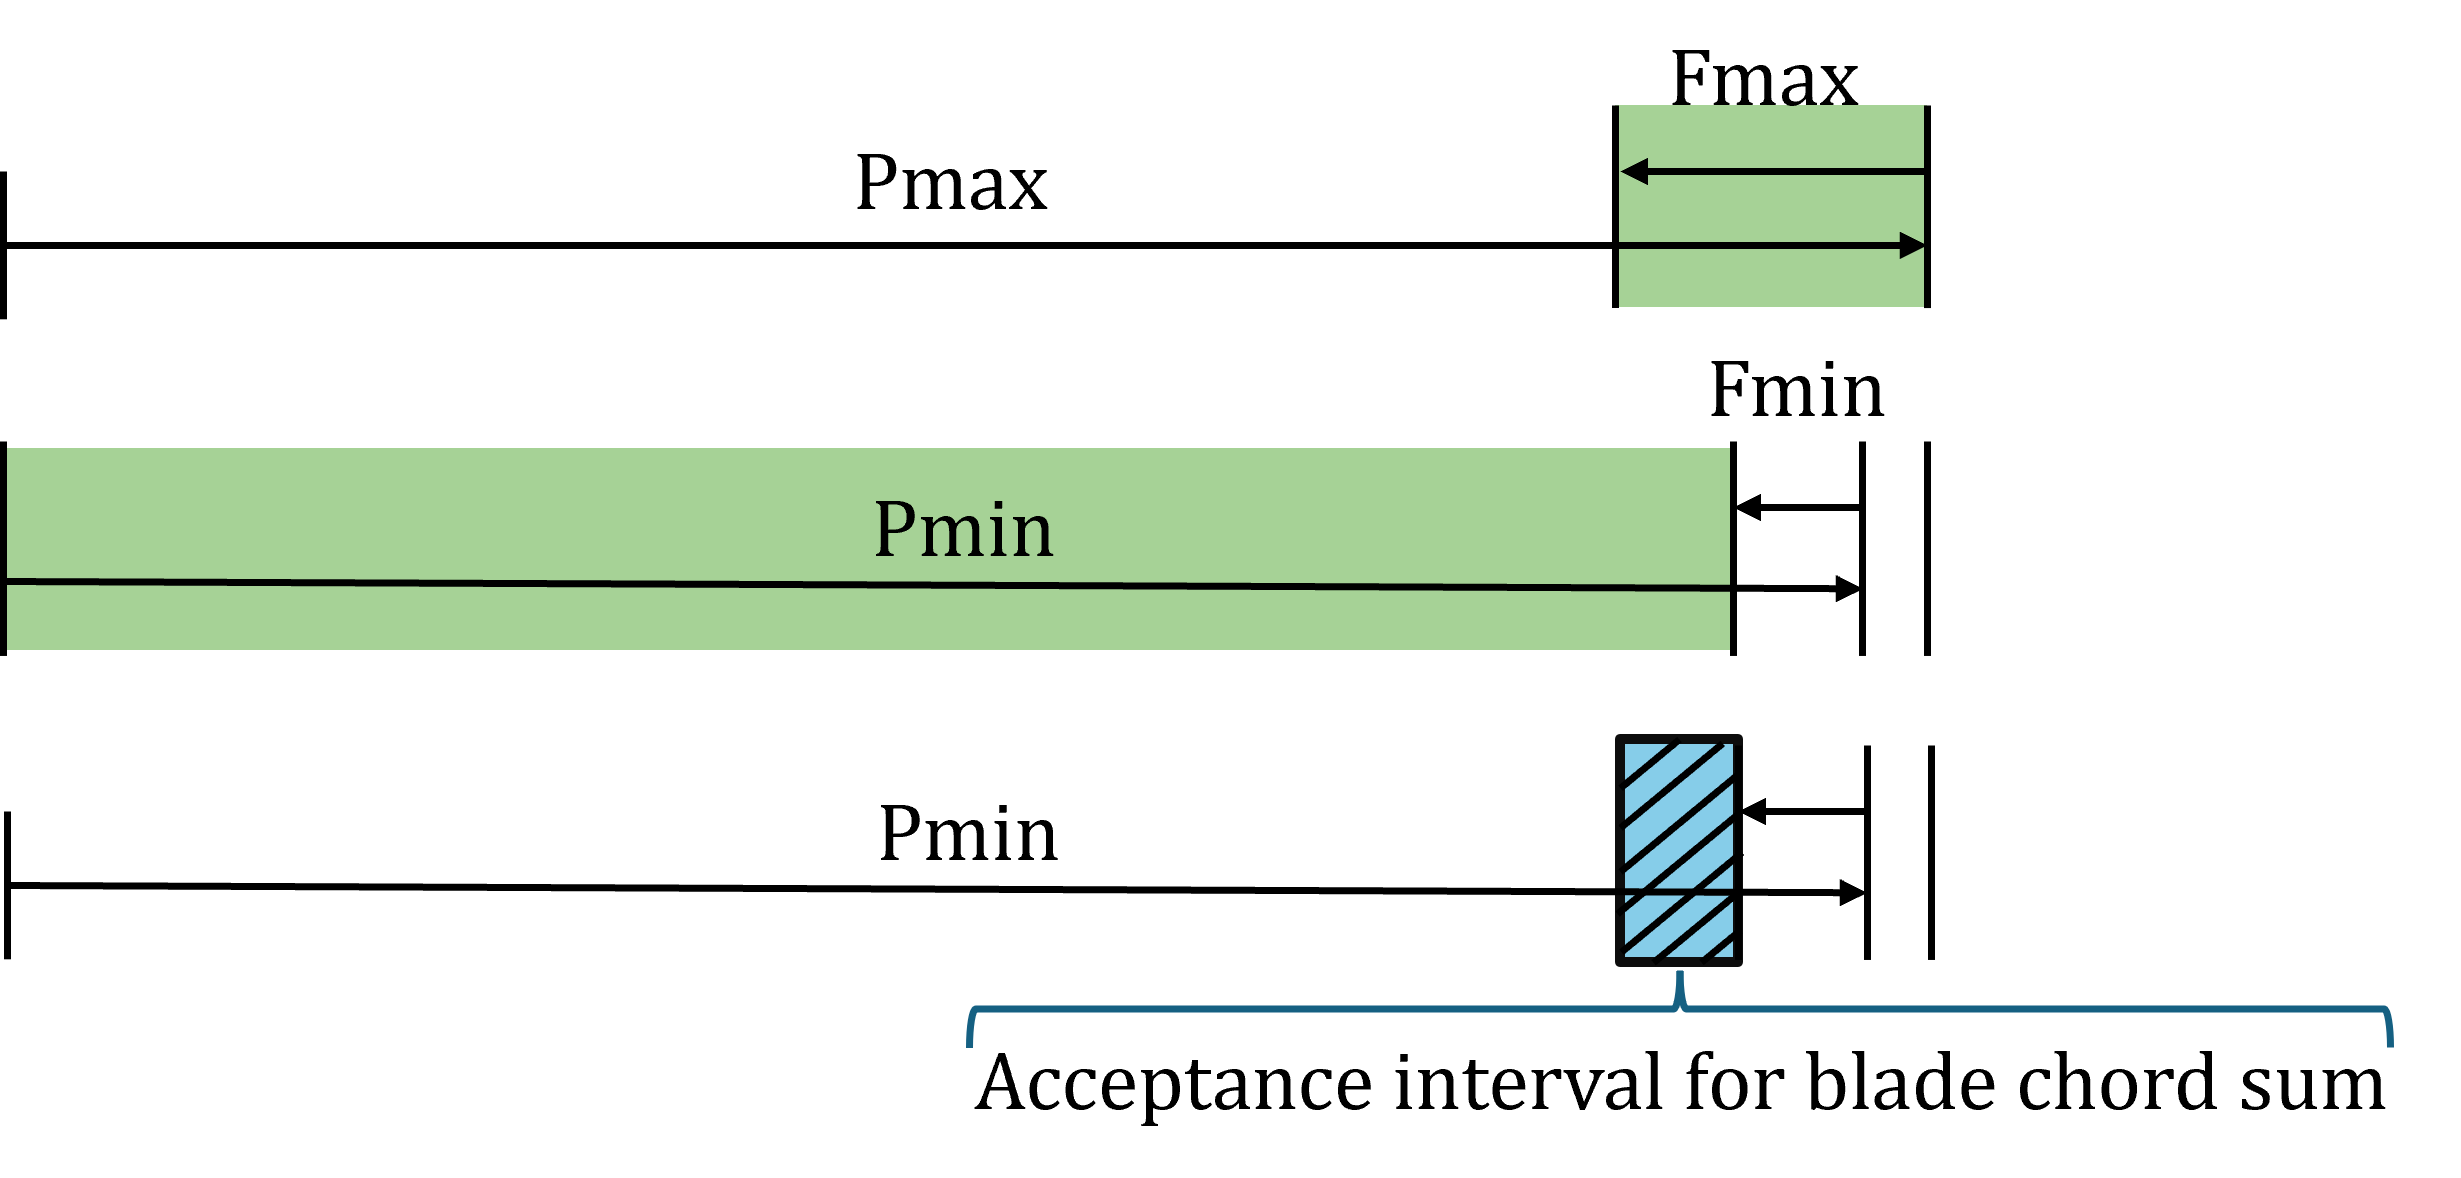
\includegraphics[width=0.75\textwidth]{imagemtolerancias}
\caption{Functional tolerance window for the total blade chord length, based on spool perimeter limits adjusted by clearance allowances and arc-to-chord transformation.}
\label{fig:imagemtolerancias}
\end{figure}

Table~\ref{tab:admissible_limits} presents the final admissible limits obtained for each stage, considering both clearance requirements and arc-to-chord transformation effects.

\begin{table}[H]
    \centering
    \caption{Admissible limits for the total blade chord length per stage}
    \label{tab:admissible_limits}
    \begin{tabular}{ccc}
        \hline
        \textbf{Stage} & \textbf{Min (mm)} & \textbf{Max (mm)} \\
        \hline
        6  & 1244.030 & 1244.479 \\
        7  & 1249.135 & 1249.582 \\
        8  & 1254.176 & 1254.624 \\
        9  & 1254.548 & 1254.996 \\
        10 & 1251.619 & 1252.068 \\
        \hline
    \end{tabular}
\end{table}

Based on all the considerations previously discussed, a first version of the tool was developed as a single-piece component.

The tolerances applied to the defined fit for the slots are shown in Figure~\ref{fig:calhav1}, which provides an overall view of the tool. The detailed technical drawing of the slot is presented in Figure~\ref{fig:anexo_2d_calhav1}.

\begin{figure}[H]
\centering
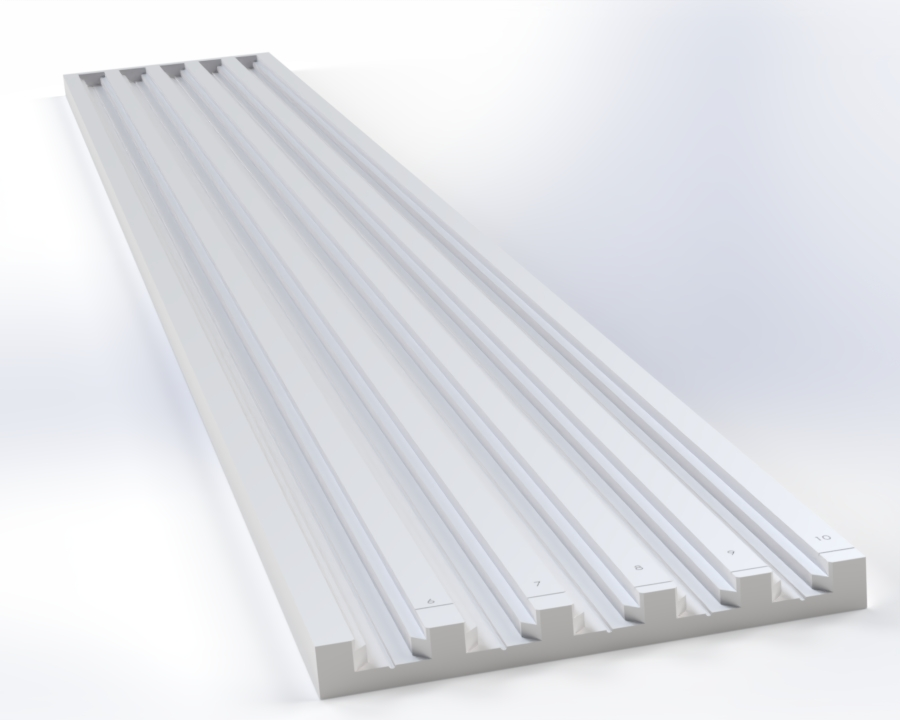
\includegraphics[width=0.75\textwidth]{calhav1}
\caption{First Tool Design.}
\label{fig:calhav1}
\end{figure}


\section{Prototype Manufacturing}

Following the definition of the final geometry and tolerances for the tool, the next step involved the construction of a physical prototype. 
The aim was to validate the design assumptions and assess the feasibility of the manufacturing process, as well as the functionality of the tool in practical terms.

To initiate the validation phase, an initial prototype was produced using 3D printing in PLA. This 3D-printed model served primarily as a physical reference to analyse the fit and assembly of the blades within the tool body. It also allowed for a preliminary assessment of the channel geometry, helping to visualise its trajectory and anticipate potential challenges during CNC machining, particularly in relation to tool accessibility and clearance.

Figure X presents the PLA prototype, while Figure Y illustrates the assembly of the blades onto the 3D-printed tool. 
This tangible analysis enabled the identification of critical areas requiring design adjustments to accommodate the constraints of the milling process.

Following this evaluation, a revised 2D technical drawing was produced, incorporating specific modifications under a design-for-manufacturing (DFM) approach. 
These changes included adjustments to the internal radii and geometrical simplifications, ensuring compatibility with standard end mill dimensions and improving the overall manufacturability of the component.









